

% Set up the document
\documentclass[convert={density=300,size=1080x800,outext=.png}]{standalone}

% Include any extra LaTeX packages required
%\usepackage[square, numbers, comma, sort&compress]{natbib}  % Use the "Natbib" style for the references in the Bibliography

\usepackage{verbatim}  % Needed for the "comment" environment to make LaTeX comments
\usepackage[table,x11names]{xcolor} % needed for highlighted rows

\usepackage{tabularx,booktabs,adjustbox} % For tables
\usepackage{pdflscape} % For writing some pages in landscape mode
\usepackage{afterpage} % For control over the positioning of figures and tables.

% For pictures
\usepackage{tikz}
\usetikzlibrary{calc,fit,arrows,decorations.pathmorphing,backgrounds,fit,positioning}
\usetikzlibrary{shapes.symbols}

% tikz colour settings
\tikzset{pop0/.style={red!70},pop1/.style={blue!70},pop2/.style={teal!70}}

%% ----------------------------------------------------------------
\begin{document}
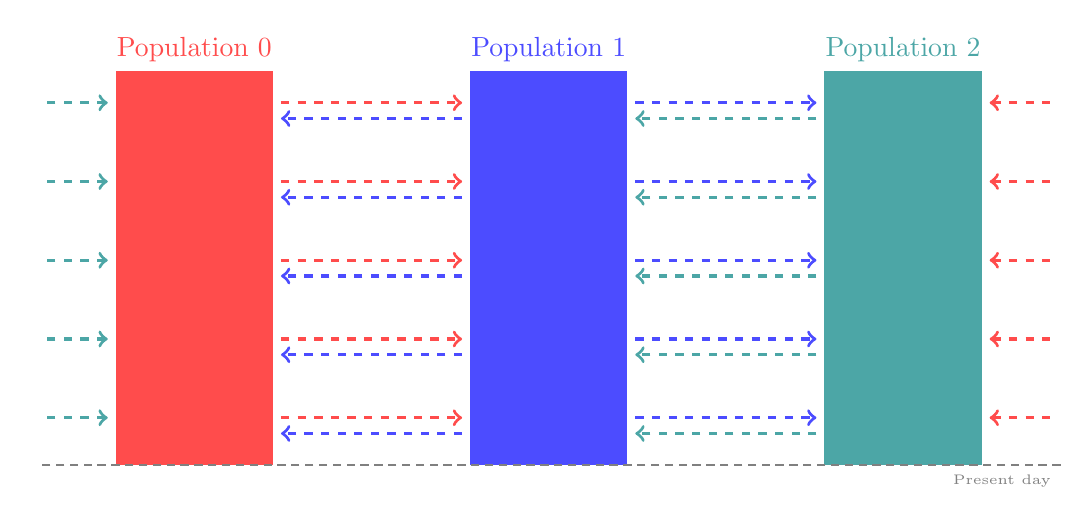
\begin{tikzpicture}[node distance=5mm and 5mm]

\tikzset{greynode/.style={font=\footnotesize,node distance=1cm and 1 cm,fill=black!10,draw=black!30,inner sep=0pt,minimum size=3.5mm,shape=circle},
mutations/.style={shape=starburst,fill=red!50!blue,inner sep=0.8pt,starburst points=11,starburst point height=.2cm}}

% Nodes
\node (origin) at (0,0){};
\node (pop0) at (1,0){};
\node (pop1) at (5.5,0){};
\node (pop2) at (10,0){};
\node (popwidth) at (2,0){};

% Axis
\node (leftAx) at (-1,0) {};
%\draw[very thick,->] (-1,0) -- +(0, 5.5);
%\foreach \y in {0, 1, 2, 3, 4, 5} \draw ($(leftAx) + (-0.1, \y)$) -- ($(leftAx) + (0.1, \y)$); % tick marks
%%\node[anchor=east] at ($(leftAx)$) {0}; \node[anchor=east] at ($(leftAx) + (0,5)$) {5};
%\node[rotate=90,anchor=south] (leftLabel) at ($(leftAx) + (-0.3,2.5)$) {$\textrm{Time}$};

% Populations
\foreach \x in {0,1,2} \fill[pop\x] ($(leftAx) + (pop\x)$) -- ++(0,5) -- ++(2, 0) -- ++(0, -5) -- cycle;
\foreach \x in {0,1,2} \node[above,pop\x] (label\x) at ($(leftAx) + (pop\x) + (1, 5)$) {Population \x};

% Migrations
\foreach \y in {0,1,2,3,4} \draw[pop0,dashed,->,very thick] ($(.1,.1) + (leftAx) + (0,\y + .5)+(pop0) + (popwidth)$) -- +(2.3,0);
\foreach \y in {0,1,2,3,4} \draw[pop1,dashed,->,very thick] ($(-.1,-.1) + (leftAx) + (0,\y + .5)+(pop1)$) -- +(-2.3,0);
\foreach \y in {0,1,2,3,4} \draw[pop1,dashed,->,very thick] ($(.1,.1) + (leftAx) + (0,\y + .5)+(pop1) + (popwidth)$) -- +(2.3,0);
\foreach \y in {0,1,2,3,4} \draw[pop2,dashed,->,very thick] ($(-.1,-.1) + (leftAx) + (0,\y + .5)+(pop2)$) -- +(-2.3,0);
\foreach \y in {0,1,2,3,4} \draw[pop0,dashed,<-,very thick] ($(.1,.1) + (leftAx) + (0,\y + .5) + (pop2) + (popwidth)$) -- +(.8, 0);
\foreach \y in {0,1,2,3,4} \draw[pop2,dashed,<-,very thick] ($(-.1,.1) + (leftAx) + (0,\y + .5) + (pop0) $) -- +(-.8, 0);
% Times
\draw[densely dashed,color=gray] (12,0) node[below left] {\tiny Present day} -- (-1,0);

\end{tikzpicture} 
\end{document}  % The End
%% ----------------------------------------------------------------